% ============================================================================
% Example manuscript (Physical Review A style) for the project template.
% Build:  make            (latexmk -> main.pdf)
% ============================================================================
\documentclass[aps,pra,reprint,amsmath,amssymb,floatfix]{revtex4-2}

\usepackage{graphicx}
\usepackage{bm}
\usepackage{braket}

\begin{document}

\title{Rabi dynamics of a driven two-level system: a template manuscript}

\author{Andrei Tsypilnikov}
\affiliation{Instituto de F\'isica, Universidade Federal Fluminense,
Av.\ Gal.\ Milton Tavares de Souza s/n, Gragoat\'a,
24210-346 Niter\'oi, Rio de Janeiro, Brazil}

\date{\today}

\begin{abstract}
We present a minimal worked example used as the manuscript template for the
group's research projects. A single two-level system evolves under the
Hermitian off-diagonal coupling $\hat H = \omega\,\hat\sigma_x$, starting from
the excited state $\ket{\uparrow}$. The Schr\"odinger equation is solved both
analytically and numerically (a fourth-order Runge--Kutta integrator in
Fortran and Python, cross-checked symbolically in Mathematica), reproducing
the textbook Rabi oscillations $P_\downarrow(t)=\sin^2(\omega t)$. The document
illustrates the expected sectioning, equation, figure, and bibliography
conventions.
\end{abstract}

\maketitle

\section{Model}
\label{sec:model}

We consider a single qubit with basis states $\ket{\uparrow}$ and
$\ket{\downarrow}$~\cite{Sakurai2017, NielsenChuang2010}. The starting point is the off-diagonal coupling
$\omega\ket{\uparrow}\!\bra{\downarrow}$; its Hermitian completion is
\begin{equation}
  \hat H = \omega\bigl(\ket{\uparrow}\!\bra{\downarrow}
        + \ket{\downarrow}\!\bra{\uparrow}\bigr)
        = \omega\,\hat\sigma_x ,
  \label{eq:hamiltonian}
\end{equation}
with $\omega$ a real coupling rate and $\hbar = 1$. We take the initial state
to be the excited state, $\ket{\psi(0)} = \ket{\uparrow}$.

\section{Exact solution}
\label{sec:exact}

Since $\hat H$ is time independent, the state evolves as
$\ket{\psi(t)} = e^{-i\hat H t}\ket{\psi(0)}$. Using
$e^{-i\omega t\,\hat\sigma_x} = \cos(\omega t)\,\hat{\mathbb{1}}
- i\sin(\omega t)\,\hat\sigma_x$, we obtain
\begin{equation}
  \ket{\psi(t)} = \cos(\omega t)\,\ket{\uparrow}
                - i\sin(\omega t)\,\ket{\downarrow} .
  \label{eq:state}
\end{equation}
The population of the lower level and the inversion are
\begin{align}
  P_\downarrow(t) &= |\!\braket{\downarrow|\psi(t)}\!|^2 = \sin^2(\omega t),
  \label{eq:pdown}\\
  \braket{\hat\sigma_z}(t) &= P_\uparrow(t) - P_\downarrow(t)
                            = \cos(2\omega t),
  \label{eq:sigmaz}
\end{align}
i.e.\ Rabi oscillations at angular frequency $2\omega$~\cite{Rabi1937}.

\section{Numerics}
\label{sec:numerics}

Equation~\eqref{eq:hamiltonian} is integrated with the classical fourth-order
Runge--Kutta scheme applied to $d\ket{\psi}/dt = -i\hat H\ket{\psi}$. The same
algorithm is implemented in Fortran (\textsc{fpm} package \texttt{two\_level})
and in Python (package \texttt{two\_level}); a Mathematica script provides an
independent symbolic check of Eqs.~\eqref{eq:state}--\eqref{eq:sigmaz}. The
numerical trajectories reproduce the analytic result to machine precision over
the integration window, as shown in Fig.~\ref{fig:dynamics}.

\begin{figure}[t]
  \centering
  % Generated by numerics/python/run.py -> results/two_level_dynamics.png
  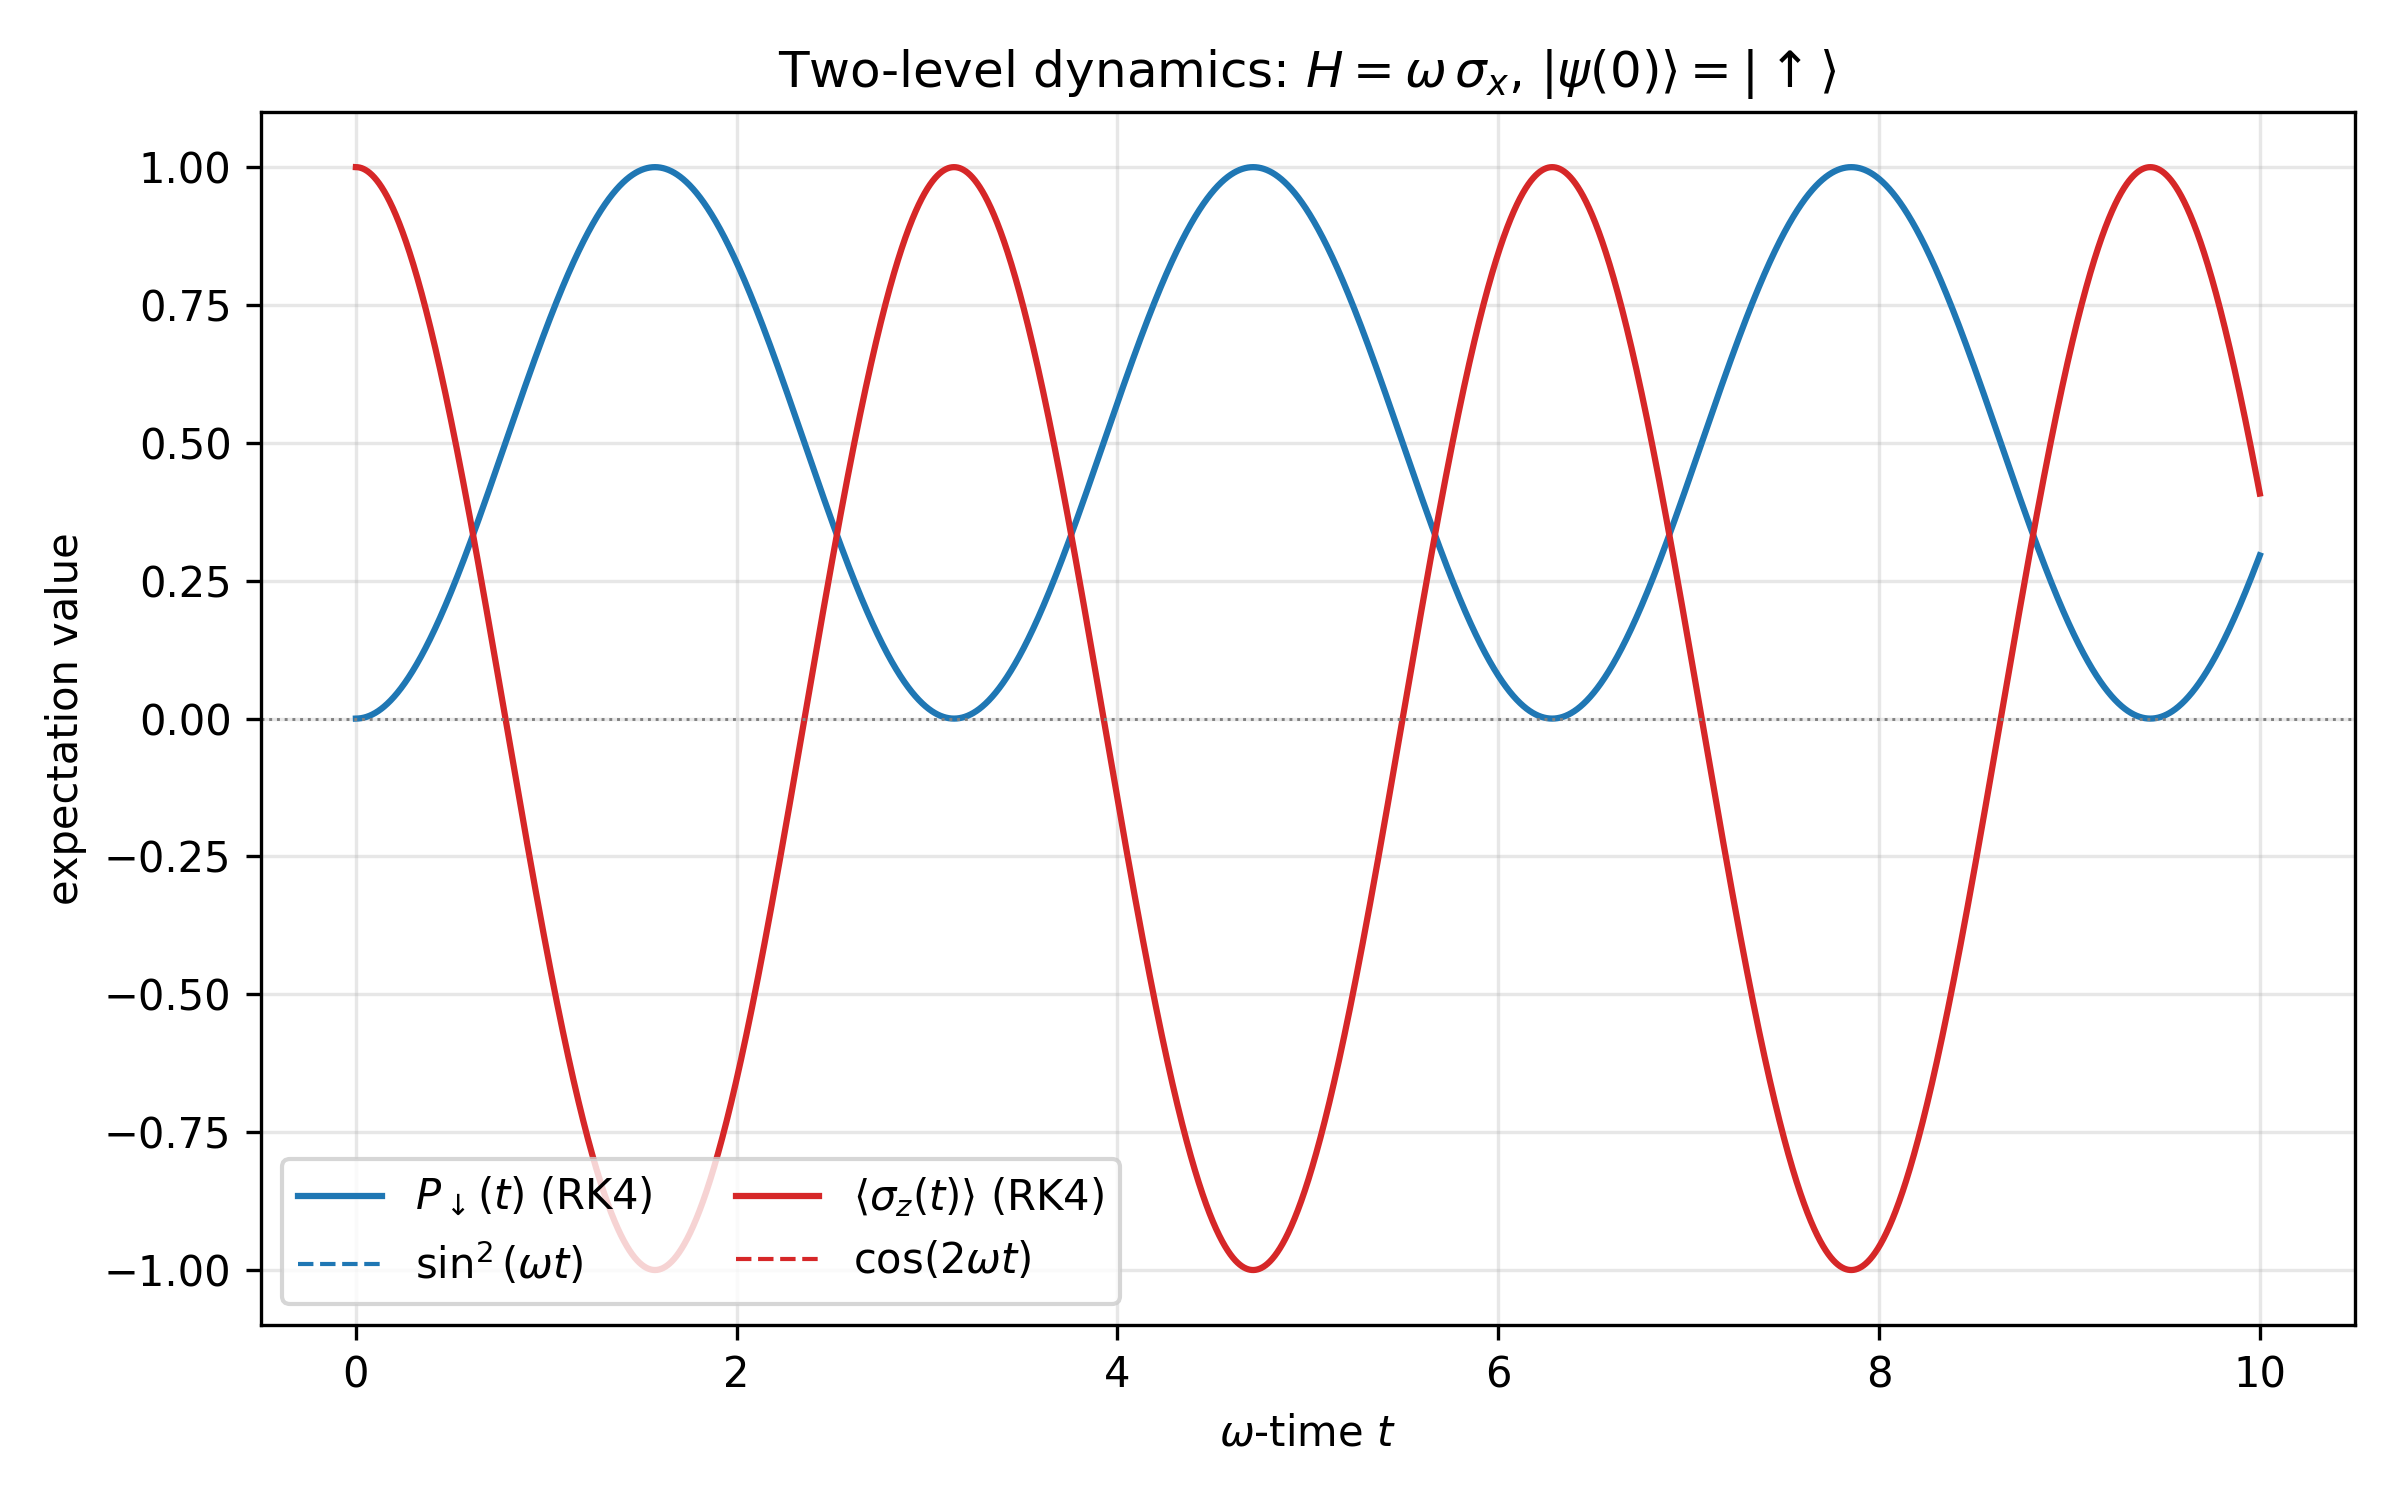
\includegraphics[width=\columnwidth]{figs/two_level_dynamics.png}
  \caption{Two-level dynamics for $\hat H = \omega\,\hat\sigma_x$ with
  $\ket{\psi(0)} = \ket{\uparrow}$: numerical RK4 (solid) versus the analytic
  Rabi solution of Eqs.~\eqref{eq:pdown}--\eqref{eq:sigmaz} (dashed). Replace
  this placeholder with the figure produced by the numerics.}
  \label{fig:dynamics}
\end{figure}

\section{Conclusion}
\label{sec:conclusion}

This template reproduces the analytically known Rabi dynamics of a single
qubit and serves as the starting point for new projects, wiring together a
LaTeX manuscript, step-by-step theory notes, and cross-validated Fortran,
Python, and Mathematica numerics.

\begin{acknowledgments}
This work was supported by the Instituto de F\'isica, Universidade Federal
Fluminense.
\end{acknowledgments}

\bibliography{biblio}

\end{document}
